\section{Comparing Models on the Complete Signal Grid}\label{sec:FS}
So far in the analysis I have only tested on a subset of the signal grid, which I have called the original signal grid. In this section 
I will extend my search to include the complete signal grid displayed in figure \ref{fig:nrSignal}. The full grid consists of 89 mass 
combinations compared to the original 30, and extends the mass ranges to $\tilde{\chi}_1 \in [0-400]$GeV and $\tilde{\chi}_2 \in [200-800]$GeV.
In the figures to come, I have included a turquoise band around all points for which a significance of more than 1.64 is expected (see section \ref{subsec:Sensitivity}).
When comparing the results, we are not only interested in how sensitive the models are for each combination individually, but also for how many points we are 
able to achieve a sensitivity over 1.64. However, similarly to previous results, the significance does not include any uncertainty.
\\
I will not apply all previously tested models to the complete signal grid. Instead, I will only apply the models I found most ideal for this analysis, based 
on the tests performed in the previous sections. I decided to choose one model from each 'type'\footnote{By network type, I am referring to either the ordinary dense network, the 
\ac{PNN} or a \ac{LWTA} model. } of network. Based on the results in section \ref{sec:Ensemble}, where I compared the different ensemble methods, I found the maxout model to be 
the top performer. Likewise, in section \ref{sec:PCA}, I found that both maxout and the \ac{PNN} preferred to utilize data with \ac{PCA}. Therefore, I will utilize the maxout model 
and \ac{PNN} model defined in section \ref{subsec:arch} with the use of \ac{PCA}. Finally, I will include the ordinary dense \ac{NN}, but without a \ac{PCA}, 
as this was found to be preferred.
\\
In figure \ref{fig:NN_FS_MLMGridSig} I have drawn a grid displaying the sensitivity of an ordinary dense \ac{NN}, on the complete signal grid. Again, we observe that higher statistics
mass combinations, result in a higher significance. Additionally, the dense \ac{NN} was able to achieve a sufficient significance for over 38 mass combinations, all between the ranges of 
$\tilde{\chi}_1 \in [0-250]$GeV and $\tilde{\chi}_2 \in [200-600]$GeV. What is even more interesting, is that by comparing the results on the full set with the results on the original 
set (see figure \ref{fig:NNGridSig}), we notice that the network was able to improve its sensitivity on every single mass combination from the original signal set. This is yet another 
indication that the deep networks are able to exploit overlapping regions in the feature space between nearby combinations.\\
\begin{figure}
    \makebox[\linewidth][c]{%
    \centering
    \begin{subfigure}{.85\textwidth}
        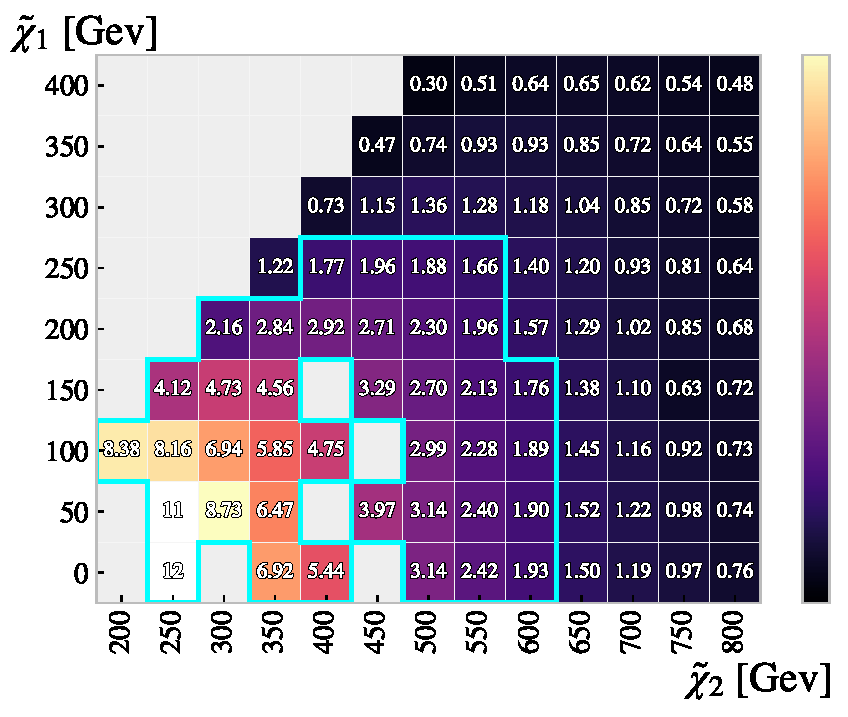
\includegraphics[width=\textwidth]{Figures/MLResults/NN/SUSY/Grid/FS/NN_FS_MLMGridSig.pdf}
    \end{subfigure}
    }
    \caption{A grid displaying the expected significance on the complete signal grid, using the signal region 
    created by the \acs{NN}. A band around each cell with a significance over 1.64 has been included.}
    \label{fig:NN_FS_MLMGridSig}
\end{figure}
Figure \ref{fig:MaxOutPCA_FS_MLMGridSig} displays a grid presenting the sensitivity of the maxout model using the complete signal grid.
The data used to train this model, has been through a \ac{PCA}, and the architecture is the same as described in section \ref{subsec:arch}.
Similarly to the dense \ac{NN}, by including the complete grid, the maxout model improved performance on all combinations in the original set. 
Also, the maxout model achieves a significance over the limit ($>1.64$) for the same mass combinations as the dense \ac{NN}. However, contrary to the tests 
performed on the original signal set, the dense network outperforms the maxout model for most of the signals points (74 out of 89 mass combinations) when 
using the full signal grid. A possible explanation to the shift in performance could be that the dense \ac{NN} lacked the statistics when training 
with the original signal set. When the complete signal grid is included, the dense \ac{NN} (which is deeper than the maxout model) is able to train 
much deeper, which in tern, increases sensitivity. However, the maxout model outperforms the dense network for the low statistics combinations, again 
indicating the maxout layers ability to increase long-term memory.\\
\begin{figure}
    \makebox[\linewidth][c]{%
    \centering
    \begin{subfigure}{.85\textwidth}
        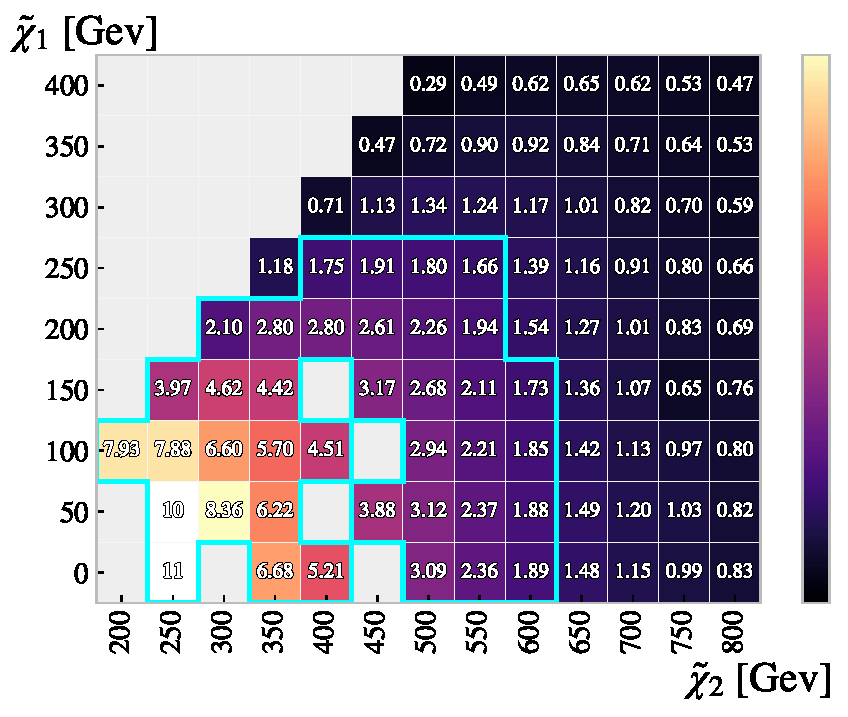
\includegraphics[width=\textwidth]{Figures/MLResults/NN/SUSY/Grid/FS/MaxOutPCA_FS_MLMGridSig.pdf}
    \end{subfigure}
    }
    \caption{A grid displaying the expected significance on the full statistics signal set, using the signal region 
    created by the maxout network. A band around each cell with a significance over 1.64 has been included.}
    \label{fig:MaxOutPCA_FS_MLMGridSig}
\end{figure}
Finally, I applied the \ac{PNN} to the complete signal grid. The results are found in the grid presented in figure \ref{fig:PNNPCA_FS_MLMGridSig}.
Similarly to the tests performed with the original signal set, the \ac{PNN} is able to achieve a high sensitivity for the high statistics mass combinations
($\tilde{\chi}_2<400$GeV). For the combinations with the highest statistics ($\tilde{\chi}_2<300$GeV), the \ac{PNN} more than doubles the expected significance of the previous 
two methods. For the lower statistics combinations, the \ac{PNN} drops in performance. Moreover, the performance of the \ac{PNN} on the combinations with the highest 
statistics in the original signal set ($\{250,400\}_{GeV}$ and $\{200,450\}_{GeV}$), has decreased by more than half.
This is an indication that including further trends in the data was destructive for training. In other words, although the \ac{PNN} achieves impressive sensitivity towards high 
statistics mass combinations, it suffers from the lack of long-term memory which allows the maxout model to uphold performance for lower statics combinations. In the appendix 
(\ref{appendix:BigVsSmall}) I have included two pie-plots comparing the performance of the maxout model and \ac{PNN} (figures \ref{fig:BigVsLittleSetMaxOut} and \ref{fig:BigVsLittleSetPNN} 
respectively) on the original signal set using models trained on the original and the complete signal grid, respectively. The 'pie-plots' further exemplify how the maxout model is able to exploit 
the full statistics to improve on most mass combinations (17/30), compared to the \ac{PNN} where the performance drops for most combinations (28/30). Finally, in comparison to the ordinary 
dense network and the maxout model which both achieved sufficient sensitivity for 38/89 combinations, the \ac{PNN} only did so for 33/89.\\
\begin{figure}
    \makebox[\linewidth][c]{%
    \centering
    \begin{subfigure}{.85\textwidth}
        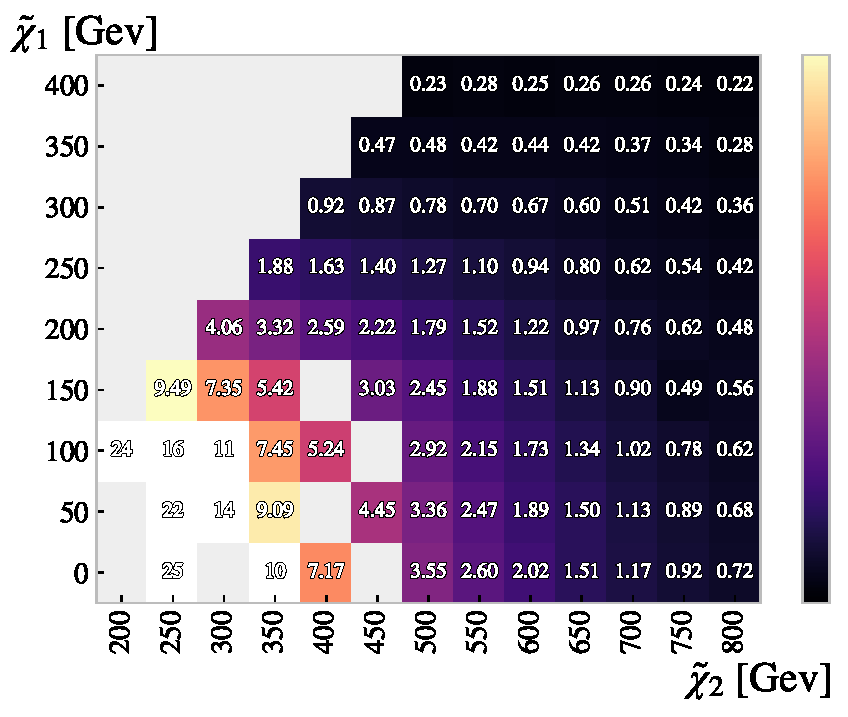
\includegraphics[width=\textwidth]{Figures/MLResults/NN/SUSY/Grid/FS/PNNPCA_FS_MLMGridSig.pdf}
    \end{subfigure}
    }
    \caption{A grid displaying the expected significance on the complete signal grid, using the signal region 
    created by the \acs{PNN} network. A band around each cell with a significance over 1.64 has been included.}
    \label{fig:PNNPCA_FS_MLMGridSig}
\end{figure}
To summarize the comparisons on the complete signal grid, I created a 'pie-plot' in figure \ref{fig:FSComp}. As shown in the figure, the ordinary dense \ac{NN}
achieved the highest sensitivity in most of the combinations (49/89), followed by the \ac{PNN} (25/89) and the maxout model (15/89). From the tests we can conclude that 
the \ac{PNN} network achieves the highest sensitivity, but struggles for unbalanced data sets. On the contrary the ordinary dense neural network performs best with larger amounts of 
training data, achieving the highest sensitivity on the largest number of combinations, but never attains the same degree of sensitivity as the \ac{PNN}. The maxout layer underperforms on 
most combinations, but exhibits impressive training memory, attaining the most balanced performance on all combinations.
\begin{figure}
    \makebox[\linewidth][c]{%
    \centering
    \begin{subfigure}{.85\textwidth}
        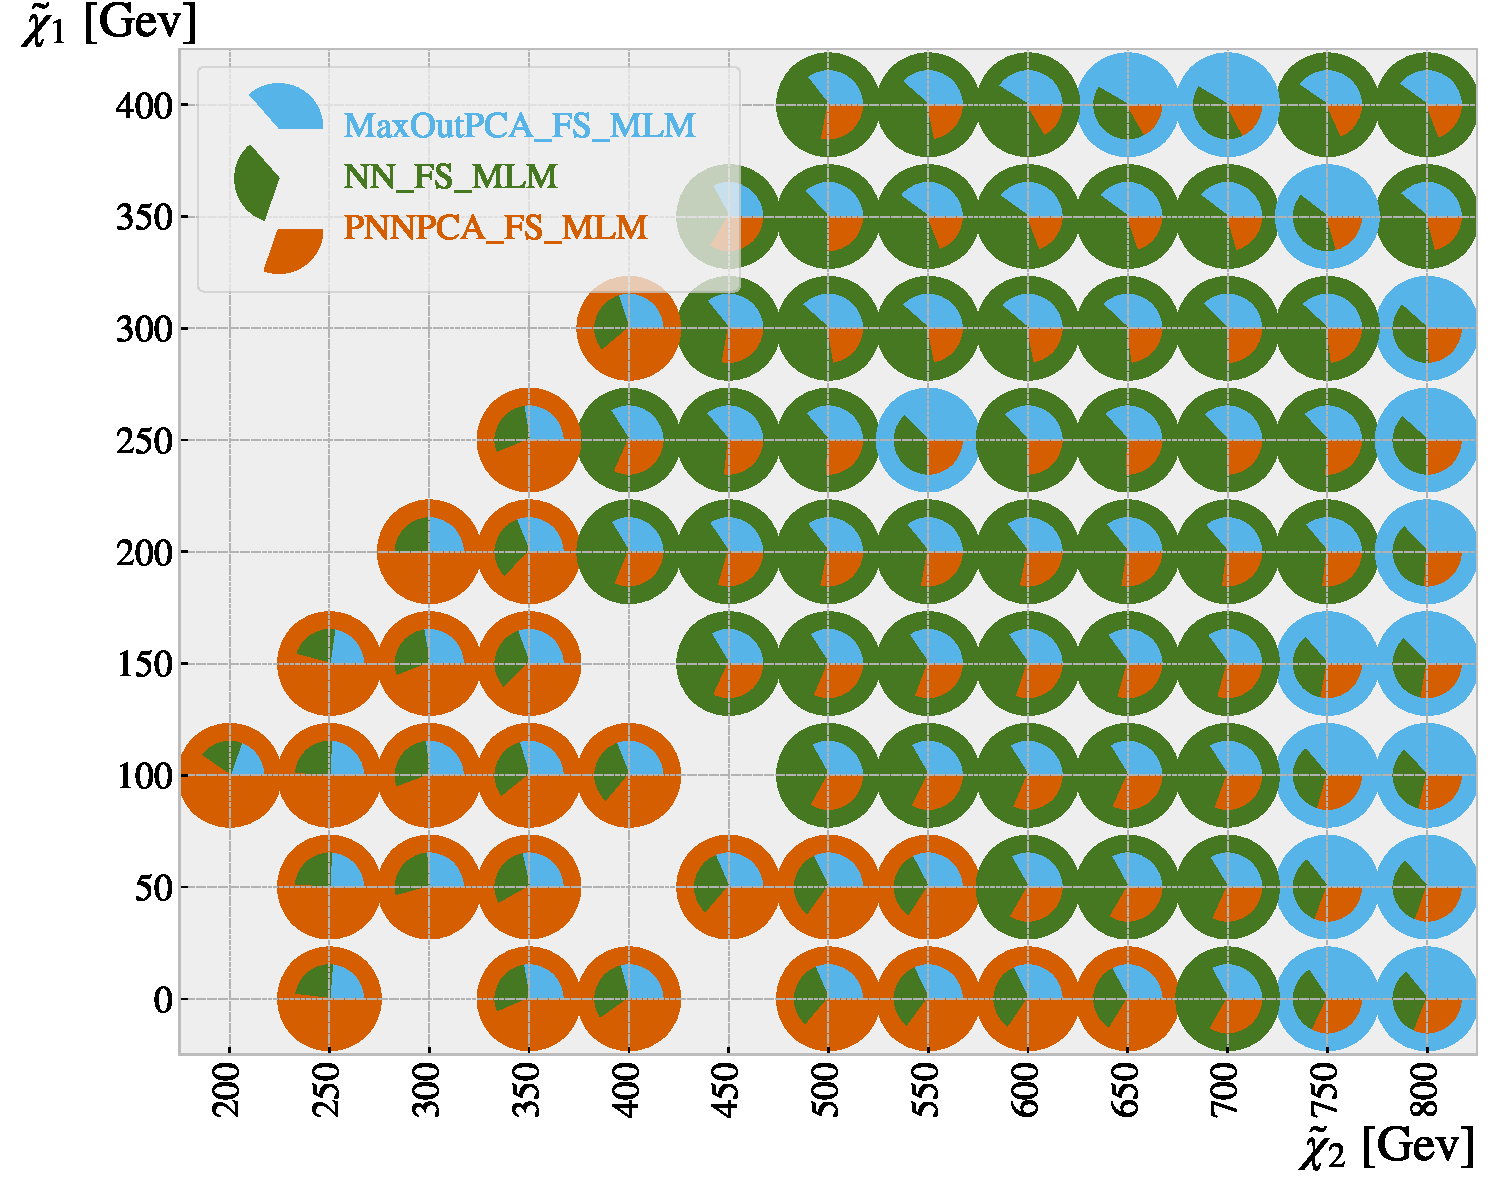
\includegraphics[width=\textwidth]{Figures/MLResults/NN/SUSY/Comparison/FS_MLMNetworkComp.pdf}
    \end{subfigure}
    }
    \caption[A sensitivity comparison between a dense \acs{NN}, \acs{PNN} and maxout on the complete signal grid.
    A \acs{PCA} analysis has been applied to the data being utilized by the latter two models.]{
    A sensitivity comparison between a dense \ac{NN}, \ac{PNN} and maxout on the complete signal grid. 
    A \ac{PCA} analysis has been applied to the data being utilized by the latter two models.
    The size of each 'slice' represents the relative size of the significance and the color around each point 
    displays the method with the largest sensitivity for the respective combination.}
    \label{fig:FSComp}
\end{figure}